\documentclass[../main.tex]{subfiles}
%\graphicspath{{\subfix{images/}}}


\begin{document}

%\section{Galois Theory (medium)}
\label{appen:galois theory}

In the previous section, we have introduced some basics about group, ring and field theories. We start this section by introducing field extension that is fundamental to understand number field. All things lead to the Galois group in the end, which is interesting in itself as well as gives insights of cyclotomic number field that is widely used across recent lattice-based cryptography and homomorphic encryption developments.  


\subsection{Field extension}
\label{subsection:field extension}
The concept of field extensions is fundamental in solving polynomials, especially polynomials with rational coefficients, denoted by $\Q[x]$. The first attempt to solve these polynomials is to find  their roots in the field of rationals $\Q$. For some rational (coefficient) polynomials, however, their roots only exist beyond $\Q$. For example, the polynomial $x^2-2$ has two irrational roots $\pm \sqrt{2}$. For this reason, we need to construct a field that is larger than $\Q$ so that it includes all roots of the polynomial $x^2-2$, but not too large that includes many unnecessary values. To achieve this goal, we first define extension fields.      

\begin{definition}
If a field $F$ is contained in a field $E$, then $E$ is called an \textbf{extension field} of $F$. 
\end{definition}
If $E$ is an extension (field) of $F$, then $F$ is a \textbf{subfield} of $E$. This pair of fields is called a \textbf{field extension} and denoted by $E/F$.\reversemarginpar
\marginnote{\textit{Field extension}}\index{field extension}

For the above example $x^2-2$, we can \textbf{adjoin} to $\Q$ the roots of this polynomial  to get a  larger field that includes all the roots of $x^2-2$, denoted by $\Q(\pm \sqrt{2}) := \{ a \pm b\sqrt{2} \,:\, a,b \in \Q\}$. Note that since an extension field is also a field, it is sufficient to adjoin only $\sqrt{2}$. Being a field also implies the extension $Q(\sqrt{2})$ includes more elements such as $1+\sqrt{2}$, $5\sqrt{2}$ and so on. 

\reversemarginpar
\marginnote{\textit{$F$-vector space}}
Given a field extension $E/F$, the larger field $E$ forms a vector space over $F$, which is also known as an \textbf{$F$-vector space}. The larger field $E$ consists of the ``vectors'' in the vector space and the smaller field $F$ consists of the scalars for multiplying with the vectors. For example, $\Q(\sqrt{2})$ forms a $\Q$-vector space, because the extension $\Q(\sqrt{2})$ is closed under addition (satisfying commutativity, associativity, additive identity and inverse) and scalar multiplication with $\Q$ (satisfying compatibility, scalar identity in $\Q$, distributivity of scalar multiplication w.r.t. scalar addition in $\Q$ or addition in $\Q(\sqrt{2})$). 

\reversemarginpar
\marginnote{\textit{Field extension degree}}
Since an extension forms a vector space over the base field, it makes sense to talk about the degree of an extension. 
\begin{definition}
Give a field extension $E/F$, the \textbf{degree} of the extension field $E$, denoted by $[E:F]$, is the dimension of the vector space formed by $E$ over $F$.
\end{definition}
An extension $E$ is \textbf{finite} if its degree is finite. Otherwise, it is infinite. 
There are at least two ways of counting the dimension of an extension. One way is through the degree of the minimal polynomial of a primitive element that generates the extension. This will be discussed in more detail in subsequent subsections. 


The other way of counting the dimension of the extension field is by counting the number of linearly independent vectors in its basis (same as for vector spaces in linear algebra). Hence, one could specify a basis of the extension over the base field in order to get the degree of the extension. For example, the degree $[\mathbb{Q}(\sqrt{2}):\mathbb{Q}]=2$,  $[\mathbb{Q}(\sqrt{2},\sqrt{3}):\mathbb{Q}]=4$, $[\C:\mathbb{R}]=2$ because the corresponding basis for each  extension field is $\{1, \sqrt{2}\}, \{1, \sqrt{2},\sqrt{3},\sqrt{6}\}, \{1,i\}$ respectively.

Similar to Lagrange's theorem in group theory, the degrees of extensions follow the ``Tower Law''. 
\begin{proposition} (The Tower Law)
\label{prop:tower law}
If $L/M$ and $M/K$ are field extensions (finite or infinite), then the degrees of the extensions satisfy 
\begin{equation*}
    [L:K] = [L:M][M:K].
\end{equation*}
\end{proposition}
Intuitively, $L$ forms a $M$-vector space and $M$ forms a $K$-vector space, so $L$ also forms a $K$-vector space. Each dimension in $L$ over $M$ is again a $[M:K]$-dimensional vector space.  

The following subsections introduce some special types of field extensions that eventually lead to Galois extensions and Galois groups. 

\subsubsection{Algebraic extension}
Historically, solving mathematical equations with rational coefficients was a natural but challenging task. This lead to the definition of algebraic numbers that are roots of non-zero rational polynomials. More formally, 

\reversemarginpar
\marginnote{\textit{Algebraic number}}
\begin{definition}
A complex number is \textbf{algebraic} (over the rationals $\mathbb{Q}$) if it is a root of a non-zero polynomial whose coefficients are rational numbers. That is, $r \in \C$ is an algebraic number if it satisfies $f(r)=0$ for some non-zero polynomial $f(x) \in \Q[x]$.
\end{definition}

All rational numbers are algebraic because they can be written in a linear equation $x-r$ for all $r \in \Q$. The irrational number $\sqrt{2}$ is algebraic because it is a root of $x^2-2$. The complex number $i$ is also algebraic because it is a root of $x^2+1$. Complex numbers that are not algebraic are called \textbf{transcendental}. In other words, transcendental numbers are not roots of any rational coefficient polynomials. For example, the number $\pi$ or $e$. 

Almost all real numbers are not algebraic. The set of real numbers is uncountable, but the set of algebraic numbers are countable. That is, there is a one-to-one correspondence between all the algebraic numbers and the natural numbers. 

When developing cryptosystems, we almost always work with integer (coefficient) polynomials $\Z[x]$. Within $\Z[x]$, monic polynomials are of special interest due to their computational efficiency. A polynomial is \textbf{monic} if the coefficient of its leading term (i.e., the term with the highest degree) is one. For example, when dividing polynomials, it is convenient to work with integer polynomials with leading coefficient one. In most cases, we work with polynomials defined over a field (e.g., $\Z_p[x]$ for prime $p$), so even if it is not monic, it can always made monic by dividing its coefficients with the leading term's coefficient. %\textcolor{red}{This is contradictory.  We say that we almost always work in $\mathbb{Z}[x]$ but then say that we almost always work over polynomials defined in a field.} KL: What I said was a bit confusing, by filed I mean Z_p, so still integer coefficients, but from a field, rather than a ring Z.

\reversemarginpar
\marginnote{\textit{Algebraic integer}}
\begin{definition}
A complex number is an \textbf{algebraic integer} if it is a root of a monic polynomial with integer coefficients. 
\end{definition}

Algebraic integers are generalization of ordinary integers which we call rational integers. 
Similar to numbers, field extensions can be algebraic or transcendental too. 

\reversemarginpar
\marginnote{\textit{Algebraic extension}}
\begin{definition}
A field extension $E/F$ is \textbf{algebraic} if every element in the extension field $E$ is algebraic. 
\end{definition}
Since all rational numbers are algebraic, a field extension $\Q(\alpha)$ is algebraic if all the additional elements are algebraic. 

All transcendental extensions are of infinite degree. For example, the transcendental extension $Q(\pi)$ has a basis $\{1, \pi, \pi^2, \pi^3, \dots\}$ of infinite linearly independent vectors. The above statement also implies that all finite extensions are algebraic. This is also proved in the following proposition.  

\begin{proposition}
\label{prop:finite implies algebra}
Every finite extension is algebraic.
\end{proposition}
\begin{proof}
Let $E$ be an extension over $F$ with a finite degree $[E:F]=n$. For an element $x \in E$, the elements $1, x, x^2, \dots, x^n \in E$ because $E$ is a field. These $n+1$ elements are also in the $n$-dimensional vector space over $F$, so must be linear dependent. Hence, there exists a set of non-zero coefficients $\{a_0,\dots,a_n\}$ such that $1+a_1 x+a_2 x^2+\cdots+a_n x^n=0$. This implies that $x$ is algebraic. 
\end{proof}


\reversemarginpar
\marginnote{\textit{Algebraic closed}}
\begin{definition}
A field $F$ is \textbf{algebraically closed} if for any polynomial $f(x) \in F[x]$, all of its roots are in the field $F$. 
\end{definition}
Obviously $\mathbb{Q}$ and $\mathbb{R}$ are not algebraically closed, but $\mathbb{C}$ is. This is the \textbf{Fundamental Theorem of Algebra}. It implies that all polynomials can be completely solved or factored into linear factors in the complex field $\mathbb{C}$. 

As mentioned earlier, given a field extension $\Q(r)/\Q$, another way of identifying the degree of the extension is by identifying the degree of the minimal polynomial of $r$ over $\Q$. To finish off this subsection, we define what minimal polynomial is.

\begin{definition}
A polynomial $f(x) \in F[x]$ is \textbf{reducible} over the field $F$ if it can be factored into polynomials with smaller degrees. Otherwise, it is \textbf{irreducible}.\reversemarginpar
\marginnote{\textit{Irreducible polynomial}}\index{irreducible polynomial}
\end{definition}

\begin{example}
Given the following polynomials over the field of rationals $\Q$: 
\begin{align*}
    f_1(x)&=x^2+4x+4=(x+2)(x+2),\\
    f_2(x)&=x^2-4=(x+2)(x-2),\\
    f_3(x)&=9x^2-3=(3x+\sqrt{3})(3x-\sqrt{3}),\\
    f_4(x)&=x^2+1=(x+i)(x-i),
\end{align*}
the polynomials $f_1(x)$ and $f_2(x)$ are reducible over $\Q$ whilst the other two are irreducible over $\Q$. The polynomials $f_3(x)$ and $f_4(x)$ are reducible over $\R$ and $\C$, respectively. The polynomial $f_4(x)$ is irreducible over $\R$.

\end{example}
%\kl{The irreducibility of a function can be check by Eisenstein’s Criterion. Details are needed?}

\begin{theorem}
\label{thm:quoRngIsField}
Let $p$ be a prime and $f(x) \in \F_p[x]$ be a monic irreducible polynomial of degree $n$. The quotient ring $\F_p[x]/f(x)$ is a field of order $p^n$. (Each polynomial in $\F_p[x]/f(x)$ has coefficients taken from the field $\F_p$ and the polynomial degree is at most $n-1$.)
\end{theorem}
% When interpreting the ring of polynomials $\F_p[x]/f(x)$, it means each polynomial in this quotient ring has coefficients taken from the field $\F_p$ and the polynomial degree is at most $n-1$. 
% We will see this notation  more often when introducing \textit{Algebraic Number Theory}, which has a different interpretation. 
% Theorem~\ref{thm:quoRngIsField} is needed when defining the underlying ring of the ring LWE problem\index{ring LWE}.
\begin{proof}
Each coset in the quotient ring $\F_p[x]/f(x)$ has the form $a_0 + a_1 x + \cdots + a_{n-1} x^{n-1}$, where $a_i \in \F_p$. So there are $p^n$ different cosets. The polynomial $f(x)$ is irreducible implies the quotient ring is also a field. 
\end{proof}


\begin{definition} 
\reversemarginpar
\marginnote{\textit{Minimal polynomial}}\index{minimal polynomial}
Let $E/F$ be a field extension. If $r$ is algebraic over $F$, its \textbf{minimal polynomial} over $F$ is the irreducible monic polynomial $f(x) \in F[x]$ of the least degree satisfying $f(r)=0$.
\end{definition}

It is necessary for $r$ to be algebraic, for otherwise it is not a root of any polynomial in $F[x]$.
%\textcolor{red}{This should follow the definition of a minimal polynomial rather than precede it.} KL: moved, thanks.

\reversemarginpar
\marginnote{\textit{Uniqueness}}
Note the minimal polynomial of an algebraic number over a base field is unique up to scalar multiplication. A simple argument is as the following. Let $J_r = \{f(x) \in F[x] \mid f(r)=0\}$ be the set of all polynomials in $F[x]$ where $r$ is a root, then $J_r$ is an ideal of the polynomial ring $F[x]$ (easy to verify). Let $p, q \in J_r$ be two monic polynomials of least degree $n > 0$, then $p-q \in J_r$ because $J_r$ is an ideal. Also $p-q$ has degree less than $n$ because $p,q$ are monic. This contradicts with $p,q$ being least degree polynomials in $J_r$, unless $p=q$.   

For different base fields, the minimal polynomial of a number could be different. Here is an example. Given the field extension $\R/\Q$, the minimal polynomial of $\sqrt{2}$ over $\Q$ is $x^2-2$ because this polynomial is monic, irreducible and has the least degree over the base field $\Q$ where $\sqrt{2}$ is a root. However, in the field extension $\R/\R$, the minimal polynomial for $\sqrt{2}$ is $x-\sqrt{2}$.

The degree of an extension $E=F(r)$ is the degree of the minimal polynomial of $r$ over $F$. This is formally proved by \Cref{thm:fieldExtEquiv} in the next subsection. In the above example, the degree $[\Q(\sqrt{2}):\Q]=2$, because the minimal polynomial of $\sqrt{2}$ over $\Q$ is $x^2-2$. 

%Minimal polynomials will be mentioned again when introducing simple extension fields. 

\subsubsection{Simple extension}

%\textcolor{red}{In cryptography, people are interested in algebraic extensions only?} There are different types of extensions, some of which are essential for building cryptosystems. They will be introduced later in order to understand Galois theory.


\reversemarginpar
\marginnote{\textit{Simple extension}}
\begin{definition}
An extension field $E$ over $F$ is \textbf{simple} if there exists an element $r \in E$ with $E = F(r)$. 
\end{definition}
The simple extension $F(r)$ is the smallest extension over $F$ that contains $F$ and $r$. The number $r$ can be either transcendental or algebraic, but we are only interested in algebraic simple extensions. 

In the previous section, we mentioned that if $r$ is an algebraic number over the base field $F$ then its unique minimal polynomial $p(x)$ always exists. 
In addition, since $p(x)$ is irreducible over $F$, the principal ideal $\langle p(x)\rangle $ is also maximal in $F[x]$. This gives us a way of building the extension field $F(r)$ from the polynomial ring $F[x]$ using the principal ideal by Proposition \ref{prop:quotRngIsField} as stated in the following theorem.  

\begin{theorem}
\label{thm:fieldExtEquiv}
Let $E/F$ be a field extension and $r \in E$ be an algebraic number over $F$ with minimal polynomial $p(x) \in F[x]$ of degree $n$, then 
\begin{enumerate}
    \item $F(r) \cong F[x] / \langle p(x)\rangle$.
    \item $\{1,r,r^2,\dots,r^{n-1}\}$ is a basis of the vector space $F(r)$ over $F$. 
    \item $[F(r):F] = deg(p)$.
\end{enumerate}
\end{theorem}
The first part of Theorem~\ref{thm:fieldExtEquiv} is a direct consequence of the First Isomorphism Theorem (Theorem~\ref{thm:first isomorphism theorem}).\index{First Isomorphism Theorem}
%The theorem says that the simple extension $F(r)$ can be built by taking the quotient of the polynomial ring $F[x]$ with the principle ideal $\langle p(x) \rangle$ generated by the minimal polynomial of an algebraic number $r \in E$. Since $p(x)$ is irreducible, the principle ideal is also a maximal ideal. By , the quotient ring $F[x]/\langle p(x) \rangle$ is a field. Proof is omitted.  \kl{introduce power basis here or later?}
%
% \reversemarginpar\marginnote{\textit{Uniqueness}}
An important observation as stated in the following corollary of the above theorem is that if two algebraic numbers have the same minimal polynomial, then the simple extensions generated by them are isomorphic. This tells us that simple algebraic extension of an algebraic number is unique. 

\begin{corollary}
Let $E/F$ be a field extension. If two algebraic numbers $\alpha, \beta \in E$ over $F$ have the same minimal polynomial in $F[x]$, then there is an isomorphism $\phi: F(\alpha) \rightarrow F(\beta)$ with $\phi |_F = I$.
\end{corollary}


\subsubsection{Splitting field}

One way of building the smallest field extension for solving a polynomial is to look at the splitting field of the polynomial. 

Solving a degree $n$ polynomial $f(x) \in F[x]$ for its roots can be done by rewriting it as the product of linear factors in an appropriate extension field $E$. That is,  
\begin{equation*}
    f(x) = c \prod_{i=1}^n (x-a_i),
\end{equation*}
where $c \in F$ is a constant and $x-a_i \in E[x]$ is a linear factor. This rewriting process is also known as \textbf{splitting} a polynomial. %Then another way of constructing the smallest field extension for solving a polynomial is by looking into its splitting field. %We can see from the previous example that it is not possible to split $x^2-2$ into linear factors in $\Q$. Hence, the following definition specifically defines the field, in which a polynomial can be split into its linear factors. 

\begin{definition}
Let $F$ be a field and $f(x) \in F[x]$ be a polynomial. The extension field $E$ is a \textbf{splitting field}\reversemarginpar
\marginnote{\textit{Splitting field}}\index{splitting field} of $f(x)$ over $F$ if
\begin{itemize}
    \item $f(x)$ splits over $E$ and 
    \item if $F \subseteq L \subsetneq E$, then $f(x)$ does not split over $L$.
\end{itemize}
\end{definition}
By definition, a splitting field of $f(x)$ is the smallest extension that contains all the roots of $f(x)$. Alternatively, we say that the extension $E$ is generated by the roots of $f(x)$. That is, if $r_1, \ldots,r_n$ are the roots of $f(x)$ and $E$ is the splitting field of $f(x)$ then $E = F(r_1, \ldots, r_n)$. For example, the extension $\Q(\sqrt{2})$ is the splitting field of $x^2-2 \in \Q[x]$, because the polynomial splits into $(x+\sqrt{2})(x-\sqrt{2})$ in it. But $\C$ is not a splitting field of $x^2-2$, because it is not the smallest. 

The following theorems state that the splitting field of a polynomial always exists and is unique up to isomorphism. 

\reversemarginpar
\marginnote{\textit{Existence}}
\begin{theorem}(Existence)
Let $F$ be a field and $f(x) \in F[x]$ be a polynomial of degree $n > 0$. Then there exists a splitting field $K$ of $f(x)$ over $F$ with degree $[K:F] \le n!$. 
\end{theorem}
The construction of a splitting field can be done by taking the quotient of $F[x]$ with the principle ideal $\langle f(x)\rangle$ where $f(x)$ is irreducible. If it is reducible, we can factor it into irreducible factors and take the same process repeatedly until $f(x)$ splits. %See Wikipedia for more details. 

\reversemarginpar
\marginnote{\textit{Uniqueness}}
\begin{theorem}(Uniqueness)
Let $\phi:F \rightarrow E$ be an isomorphism, $f(x) \in F[x]$ be a polynomial and $\phi(f(x)) \in E[x]$ be the corresponding polynomial in $E[x]$. If $K$ and $L$ are the splitting fields of $f(x)$ and $\phi(f(x))$ over $F$ and $E$ respectively, then $\phi$ extends to an isomorphism $K \cong L$.
\end{theorem}


\subsubsection{Normal extension}

Sometimes we prefer to work with an algebraic extension that includes all the roots of a polynomial, so that we do not need to adjoin more roots to the extension. For this purpose, we define the following. 


\reversemarginpar
\marginnote{\textit{Normal extension}}
\begin{definition}
An algebraic extension $E$ over $F$ is \textbf{normal} if whenever an irreducible polynomial over $F$ has a root in $E$, then it splits in $E$. 
\end{definition}
From splitting field, we know that an extension is normal if whenever it contains one root of a polynomial, it contains all roots of the polynomial. 
The most important result about normal extension is its connection with splitting field.

\reversemarginpar
\marginnote{\textit{Normal iff splitting}}
\begin{theorem}
\label{theorem:normal iff splitting}
A finite algebraic extension $E$ over $F$ is normal if and only if it is the splitting field of some polynomial $f(x) \in F[x]$.
\end{theorem}
The theorem implies that if $E$ is the splitting field of one polynomial over $F$, then it is the splitting field of every other polynomial over $F$ with one root in $E$. %In other words, a polynomial over $F$ either has no root in $E$ or splits completely in $E$. 


\subsubsection{Separable extension}

In addition to normal extensions, it is also convenient when a polynomial has distinct roots, so we do not need to worry about duplicated roots. This is especially the case when working with Galois groups that consist of automorphisms between polynomial roots. Before introducing separable extensions, we define what it means for a polynomial to be separable and how separability can be tested. 

\reversemarginpar
\marginnote{\textit{Separable polynomial}}
\begin{definition}
A polynomial over a field $F$ is \textbf{separable} if the number of its distinct roots in a splitting field is equal to the degree of the polynomial. 
\end{definition}

\begin{example}
The polynomial $x^2-2$ has two distinct roots $\pm \sqrt{2}$, so it is separable. 
The polynomial $(x^2-1)^2$ is not separable, because both roots $\pm 1$ have multiplicity 2. 
\end{example}

\reversemarginpar
\marginnote{\textit{Test separability}}
One way of testing separability is to check whether or not a polynomial is coprime with its \textit{formal derivative}\footnote{Formal derivative is similar to derivative in calculus, but for elements of a polynomial ring.}. 
\begin{lemma}
A polynomial $f(x) \in F[x]$ is separable if and only if $\gcd(f,f')=1$.
\end{lemma}
\begin{proof}
Let $K$ be the splitting field of $f(x)$ and $r \in K$ is a root of $f(x)$. The re-write the polynomial as 
\begin{equation*}
    f(x)=(x-r)^m g(x)
\end{equation*}
with $m \ge 1$ and $g(r) \neq 0$. Take the formal derivative, we get
\begin{equation*}
    f'(x) = m(x-r)^{m-1} g(x) + (x-r)^m g'(x) = (x-r)^{m-1} [mg(x) + (x-r)g'(x)].
\end{equation*}
Evaluating the second factor $mg(x) + (x-r)g'(x)$ at $r$ gives $mg(r) + 0 = 0 \iff m = 0$ because $g(r) \neq 0$.  

If $f(x)$ is separable, by definition $m = 1$ and $f'(x) = g(x) + (x-r)g'(x)$. So $f'(r) \neq 0$ and none of the two factors of $f(x)$ divides $f'(x)$. This implies they are coprime. 

If $f(x)$ is not separable, then $m > 1$ and $f'(r)=0$. Hence, $x-r$ is a common factor of $f$ and $f'$, so they are not coprime. 
\end{proof}

\begin{example}
In the examples above, $f(x)=x^2-2$ is separable, because its formal derivative $f(x)'=(x^2-2)' = 2x$ and $\gcd(f,f')=1$. If $f(x)=(x^2-1)^2$, then its formal derivative $f'(x)=((x^2-1)^2)'=4x(x^2-1)$ and $\gcd(f,f')=x^2-1$, so the polynomial $(x^2+1)^2$ is not separable. 
\end{example}

\reversemarginpar
\marginnote{\textit{Separable extension}}
\begin{definition}
An algebraic extension $E$ over $F$ is \textbf{separable} if for every element $\alpha \in E$, its minimum polynomial over $F$ is separable. 
\end{definition}

The Fundamental Theorem of Galois Theory states a correspondence between intermediate field extensions and subgroups of a Galois group. Hence, we would like to know the separability of the intermediate field extensions between a base field and a separable extension.    

\reversemarginpar
\marginnote{\textit{Intermediate extensions are separable}}
\begin{theorem}
Given field extensions $L/M/K$. If $L/K$ is separable, then the intermediate extensions $L/M$ and $M/K$ are also separable. 
\end{theorem}
%M/K is separable is trivial to prove, the proof of L/M should be easy,


\reversemarginpar
\marginnote{\textit{$char(F)=0 \implies$ separable}}
In the previous section, we stated that a field characteristic is either 0 or a prime. The following results connect the characteristic of a polynomial to its separability.

\begin{theorem}
\label{thm:minPolyIsSepInChar0Field}
Every irreducible polynomial over a field of characteristic zero is separable, and hence every algebraic extension is separable. 
\end{theorem}

\begin{proof}
Let $E/F$ be a field extension with $char(F)=0$, and $f(x) \in F[x]$ be the minimal polynomial of $\alpha \in E$ over $F$. Assuming $f(x)$ is not separable. That is, without loss of generality, there is a root $\beta$ with multiplicity 2. Then $f(\beta)=0$ and its formal derivative $f'(\beta)=0$, because $f(x)$ has a factor $(x-\beta)^2$, which becomes $2(x-\beta)$ in $f'(x)$. 

However, $f'(x)$ does not have zero coefficients, because it is over a field of zero characteristic. The fact that $f(x)$ is a minimal polynomial implies it is irreducible, and $f'(x)$ has a lower degree than $f(x)$ imply that $\gcd(f,f')=1$. Hence, there are $a,b \in F[x]$ such that $af(x)+bf'(x)=1$. Substituting $x=\beta$, we get a contradiction, so $f(x)$ cannot be non-separable. Hence, every irreducible polynomial over $F$ is separable. This implies every algebraic extension is separable and every finite extension is also separable because every finite extension is algebraic by Proposition \ref{prop:finite implies algebra}.       
\end{proof}

A similar but more general result is the following theorem. 

\begin{theorem}
\label{theorem:char prime implies separable}
Let $f \in F[x]$ be an irreducible polynomial of degree $n$. Then $f$ is separable if either of the following conditions is satisfied: 
\begin{itemize}
    \item the field $F$ has characteristic $0$ or 
    \item the field $F$ has characteristic $p$ where $p$ is prime and $p \nmid n$.
\end{itemize}
\end{theorem}
The same argument can be used here to prove the second condition. Since $f(x)$ is a degree $n$ polynomial, its formal derivative $f'(x)$ much contain a term $n a_n x^{n-1}$, in which the coefficient $n a_n \neq 0$ in the field $F$ as $char(F)=p$ is prime and $p \nmid n$. So $\gcd(f,f')=1$ and the same contradiction can be reached is $f(x)$ is assumed to be non-separable. 

The intuition behind both theorems is that if the characteristic of the field $F$ does not satisfy either condition, then the coefficients of $f'(x)$ may be all zero. So $f'(x)=0$ cannot lead to the same contradiction when assuming $f(x)$ non-separable. 

\subsection{Galois extension and Galois group}
In the preceding subsections, we have defined different types of field extensions, finite, algebraic, simple, normal and separable. This section will connect some of these extensions to an important field extension, called \textit{Galois extension} and will define the \textit{Galois groups} of Galois extensions. 

\reversemarginpar
\marginnote{\textit{Group action}}
To start with, we introduce group action on a set. One way to define a group action on a set is by the following definition. 

\begin{definition}
A group $(G,*)$ \textbf{acts} on a set $S$ if there is a map  
\begin{equation*}
    \mu:G \times S \rightarrow S
\end{equation*}
such that 
\begin{itemize}
    \item for all $s \in S$, we have $\mu(e,s)=s$,
    \item for all $x,y \in G$ and $s\in S$, we have $\mu(x * y, s) = \mu(x,\mu(y,s))$.
\end{itemize}
\end{definition}

For simplicity, we write $\mu(x,s)$ as $x(s)$. Another way of defining group action is by a group homomorphism.

\begin{definition}
A group $G$ \textbf{acts} on a set $S$ if there is a homomorphism 
\begin{equation*}
    \phi:G \rightarrow Sym(S)
\end{equation*}
from the group to the symmetric group (or the permutation group $Perm(S)$) of $S$. 
\end{definition}

In this case, we say $\phi$ is the group action of $G$ on $S$. Each element of $G$ is mapped to a certain permutation of the set $S$ by the action. For example, when the Dihedral group
\begin{equation*}
    D_4=\langle r,f\rangle=\{e,r,r^2,r^3,f,fr,fr^2,fr^3)
\end{equation*}
acts on itself, 
% \textcolor{red}{I think that this example is unnecessarily complicated. Part of the problem is that the dihedral group is playing two roles here. Is there some reason we can't use another eight-element set?},
each element in $D_4$ is mapped to a certain permutation of the set $S=D_4$. For example, the elements \textit{rotation} $r$ and \textit{reflection} $f$ correspond to the following permutations of $D_4$
% \textcolor{red}{What is the homomorphism here?  It looks like in the "rotate" map we have $\phi(g,s) = g \cdot s$ while in the "flip" line we have $\phi(g,s) = s \cdot g$. Because $D_4$ is nonabelian, these are different functions. Right?} \kl{Yes, I think this example could be a bit complicated. I realized I made a mistake by mixing the left and right action. I think one is transferable to another, so it's sufficient to consider one action in most cases. I'll see if I can make a simpler example. I think most people may consider the left action. The first homomorphism is $\phi_1: r \rightarrow (e \text{ } r)(r\text{ }r^2) (r^2\text{ }r^3) (r^3\text{ }e) (f\text{ }fr^3) (fr\text{ }f) (fr^2\text{ }fr) (fr^3\text{ }fr^2)$ and the second homomorphism is $\phi_2: f \rightarrow (e \text{ } f)(r\text{ }fr) (r^2\text{ }fr^2) (r^3\text{ }fr^3) (f\text{ }e) (fr\text{ }r) (fr^2\text{ }r^2) (fr^3\text{ }r^3)$. They are different homomorphisms.}
\begin{align*}
    r: \{e,r,r^2,r^3,f,fr,fr^2,fr^3) \mapsto \{r,r^2,r^3,e, rf=fr^3,rfr=f,rfr^2=fr, rfr^3=fr^2) \\
    f: \{e,r,r^2,r^3,f,fr,fr^2,fr^3) \mapsto \{f,fr,fr^2,fr^3,e,r,r^2,r^3).
\end{align*}
The action of $D_4$ only gives rise to certain permutes of $D_4$. In other words, there are 8 elements in $D_4$ and the symmetric group has size $|Perm(D_4)|=8!$, the homomorphism $\phi$ is injective, which we call faithful as stated next. 

\reversemarginpar
\marginnote{\textit{Faithful action}}
\begin{definition}
A group action $\phi$ of $G$ on a set $S$ is \textbf{faithful} if $\phi$ is injective. That is, for every two distinct elements $g, h \in G$, there exists an element $s \in S$ such that $g(s) \neq h(s)$. 
\end{definition}
If a group action is faithful, then we can think the group $G$ embeds into the permutation group of $S$, as in the above example of $D_4$, where each element of $G=D_4$ corresponds to a certain permutation of the set $S=D_4$.

Similarly, we can define a group $G$ acts on a ring $R$ (or a field $F$). The difference is that a ring has more algebraic structures than a set, so simple permutations of the ring elements do not necessarily preserve the ring structure. For this reason, we replace permutations by automorphisms, which are bijective ring homomorphisms between $R$ and itself. Let $\text{Aut}(R)$ be the \textbf{automorphism group} of $R$. 

\begin{definition}
An \textbf{action} of a group $G$ on a ring $R$ is a group homomorphism 
\begin{equation*}
    \phi: G \rightarrow \text{Aut}(R).
\end{equation*}
\end{definition}


\reversemarginpar
\marginnote{\textit{Fixed field}}
Some elements in the ring $R$ or field $F$ stay invariant under the action. They make up the fixed field. 

\begin{definition}
Given a field extension $E/F$ and a group action of $G$ on $E$, the \textbf{fixed field} of $E$ under the action of $G$ 
\begin{equation*}
    E^G = \{a \in E \mid g(a)=a, \forall g \in G\}.
\end{equation*}
is the set of elements in the extension field that are fixed point-wise by all automorphisms of $R$. 
\end{definition}


\reversemarginpar
\marginnote{\textit{Automorphism group}}
\begin{definition}
Let $E/F$ be a field extension. The \textbf{automorphism group} of the field extension 
\begin{align*}
    Aut(E/F) &= \{\alpha \in Aut(E) \mid \alpha(x) = x, \text{ } \forall x \in F\} \\
    &=\{\alpha \in Aut(E) \mid \alpha_F = Id_F\}
\end{align*}
is the set of automorphisms that fixes $F$ when acting on $E$.
\end{definition}
The automorphism group is a group with function composition as the group operator. It is a subgroup of the group of automorphisms of $E$, i.e., $Aut(E/F) \subseteq Aut(E)$. Now, we are ready to define the Galois group of a field extension.  

\begin{definition}
The \textbf{Galois group} of a field extension $E/F$, denoted by $Gal(E/F)$, is the automorphism group of the field extension.\reversemarginpar
\marginnote{\textit{Galois group}}\index{Galois group of a field extension}
That is, 
\begin{equation*}
    Gal(E/F):=Aut(E/F) = \{\alpha \in Aut(E) \mid \alpha_F = Id_F\}.
\end{equation*}
\end{definition}

By definition, the Galois group is a subset of the automorphism group or permutation group (or symmetric group) of the extension $E$. 

As explained in the previous section that an extension field can be viewed as a vector space over the base field, so when working with Galois groups, instead of thinking where all elements in the extension are mapped to, it is convenient to know where the basis vectors are mapped to by the automorphisms.

Let us work through some simple examples. 
\begin{example}
Let the field extension be $\Q(\sqrt{2})/\Q$. It is a 2-dimensional $\Q$-vector space with a basis $\{1,\sqrt{2}\}$. The Galois group must fix the base field, so it contains the identity map $I$. In addition, it should contain another automorphism $\sigma$ that maps $\sqrt{2}$ to another element $a$ in the extension whiling fixing $\Q$. Since $\sigma$ is an automorphism, it must satisfy $a^2=\sigma(\sqrt{2})^2=\sigma((\sqrt{2})^2)=\sigma(2)=2$. So whatever $\sigma(\sqrt{2})=a$ is, it must satisfy $a^2-2=0$ in the extension, which means $a=\pm \sqrt{2}$. Since the identity map is already included, it entails $\sigma(\sqrt{2})=-\sqrt{2}$. Hence, the Galois group $Gal(\Q(\sqrt{2})/\Q) = \{I, \sigma:\sqrt{2} \mapsto -\sqrt{2}\} \cong C_2$ which is isomorphic to the cyclic group of order 2. 
\end{example}

\begin{example}
\label{exam:galoisgroup2}
Let the field extension be $\Q(\sqrt{2},i)/\Q$. This is a 4-dimensional $\Q$-vector space with a basis $\{1,\sqrt{2},i,\sqrt{2}i\}$. The minimal polynomials over $\Q$ for $\sqrt{2}$ and $i$ are $x^2-2$ and $x^2+1$, respectively. The Galois group of the field extension contains all the automorphisms that fix $\Q$ while permuting roots in each minimal polynomial. That is, it contains a map $\tau$ that permutes $\{\sqrt{2},-\sqrt{2}\}$ and a map $\sigma$ that permutes $\{i,-i\}$.
We can identify these automorphisms as shown in Table \ref{tab:galoisgroup}. The Galois group is isomorphic to the Klein four group $V_4 = C_2 \times C_2$. 
\begin{table}[h!]
\centering
\begin{tabular}{|c|c|c|c|c|}
\hline
 & 1 & $\sqrt{2}$ & $i$ & $\sqrt{2}i$ \\ \hline
$I$ & 1 & $\sqrt{2}$ & $i$ & $\sqrt{2}i$  \\ \hline
$\sigma$ & 1 & $\sqrt{2}$ & $-i$ & $-\sqrt{2}i$ \\ \hline
$\tau$ & 1 & $-\sqrt{2}$ & $i$ & $-\sqrt{2}i$ \\ \hline
$\sigma \tau$ & 1 & $-\sqrt{2}$ & $-i$ & $\sqrt{2}i$ \\ \hline
\end{tabular}
\caption{The Galois group of the extension $\Q(\sqrt{2},i)$. It is isomorphic to the Klein four group $V_4=C_2\times C_2$.}
\label{tab:galoisgroup}
\end{table}
\end{example}

It is important to note that not all automorphisms (or permutations) that fix the base field are in the Galois group. From the above two examples, we can see that the Galois group only contains those automorphisms that permute roots of the same minimal polynomial while fixing the base field. In Example \ref{exam:galoisgroup2}, $\sqrt{2}$ and $-\sqrt{2}$ come from the minimal polynomial $x^2-2$ in $\Q$ and $i$ and $-i$ come from the minimal polynomial $x^2+1$ in $\Q$. Let us take a look at a counter example. 

\begin{example}
Let the field extension be $\Q(\sqrt{2},\sqrt{3})/\Q$. The permutation $\phi:\sqrt{2} \mapsto \sqrt{3}$ is not in the Galois group. Assuming it is, then $\phi(\sqrt{2}) = \sqrt{3}$ implies $\phi(\sqrt{2})^2 = 3$. By the definition of homomorphism, $\phi(\sqrt{2})^2 = \phi(\sqrt{2}^2)=\phi(2)=2$ because $\phi$ fixes $\Q$. This implies $2=3$. 
\end{example}

\begin{example}
A slightly more complicated example is with a field extension $\Q(\sqrt[4]{2},i)/\Q$. The roots $\sqrt[4]{2}$ and $i$ have the minimal polynomials $x^4-2$ and $x^2+1$ over $\Q$, respectively. The polynomial $x^4-2$ has four roots $\pm \sqrt[4]{2}$ and $\pm i\sqrt[4]{2}$. The polynomial $x^2+1$ has two roots $\pm i$. The Galois group should contain automorphisms that permutes roots for each polynomial. The process of finding the automorphisms is more or less trial and error.\footnote{Perhaps there are better ways of finding the Galois group, but they are not in the scope of this material.} Let 
\begin{align*}
    \sigma(\sqrt[4]{2}) &= i\sqrt[4]{2} \text{ and } \sigma(i)=i,\\
    \tau(i)&=-i \text{ and } \tau(\sqrt[4]{2})=\sqrt[4]{2}.
\end{align*}
Then we have 
\begin{align*}
    \sigma^2(\sqrt[4]{2}) &= -\sqrt[4]{2} \text{ and } \sigma^2(i)=i,\\
    \sigma^3(\sqrt[4]{2}) &= -i\sqrt[4]{2} \text{ and } \sigma^3(i)=i,\\
    \sigma^4(\sqrt[4]{2}) &= \sqrt[4]{2} \text{ and } \sigma^4(i)=i,\\
    \tau^2(i)&=i \text{ and } \tau^2(\sqrt[4]{2})=\sqrt[4]{2}.
\end{align*}
So the orders of $\sigma$ and $\tau$ in the Galois group are 4 and 2, respectively. Hence, the Galois group is $\{I, \sigma,\sigma^2,\sigma^3,\tau,\sigma\tau,\sigma^2\tau,\sigma^3\tau\}$.
\end{example}

Combining the definitions of fixed field and Galois group, we know that for a field extension $E/F$, the fixed field by the Galois group %$E^{Gal(E/F)} = \{a \in E \mid g(a) = a, \forall g \in Gal(E/F)\}$ 
should at least contain the base field $F$. Because all automorphisms in the Galois group at least fix $F$, though they may fix more than $F$. 
Hence, we can define what it means for a field extension to be Galois. 

\reversemarginpar
\marginnote{\textit{Galois extension}}
\begin{definition}
A field extension $E/F$ is an \textbf{Galois extension} if the fixed field by the Galois group $Gal(E/F)$ is exactly $F$. That is, $E^{Gal(E/F)} = F$.
\end{definition}

In other words, the Galois group has to fix exactly the base field, nothing more nothing less. An important theorem that characterizes Galois extension using previously defined extension types is the following. 

\reversemarginpar
\marginnote{\textit{Normal and separable $\implies$ Galois}}
\begin{theorem}
\label{theorem:separable and normal implies galois}
An algebraic field extension is a \textbf{Galois extension} if it is normal and separable. 
\end{theorem}
This theorem says that for an algebraic field extension to be a Galois extension, any polynomial that has a root in the extension must have all its roots in the extension and these roots must be all distinct. The requirement of being normal and separable is a sufficient condition for a field extension to be Galois. %That is, the Galois group $Gal(E/F)$ (i.e., collection of automorphisms between $E$) only fixes the base field $F$, nothing else.  

\begin{example}
The Galois group $Gal(\Q(\sqrt[3]{2})/\Q) = \{I\}$ contains only the identity map. If $\phi(\sqrt[3]{2})=a$ is another automorphism, then it must satisfy $a^3-2=0$. So $\phi$ must map $\sqrt[3]{2}$ to a root of the minimal polynomial $a^3-2=0$ in the extension. But the only root that is in the extension is $\sqrt[3]{2}$, because the other two roots are complex. So $\phi$ is the identity map. Given the Galois group contains only the identity map, the fixed field is $\Q(\sqrt[3]{2})$ not $\Q$, so the field extension is not Galois. By Theorem \ref{theorem:separable and normal implies galois}, the extension is not both normal and separable. In fact, this is true, because the extension does not contain the two complex roots of the minimal polynomial $x^3-2$.
\end{example}

The example suggests that a field extension can have a Galois group, but it is not necessarily a Galois extension. 

Since a Galois extension is normal and separable, we would expect the number of automorphisms in the Galois group to be related to the number of roots of a minimal polynomial. The next lemma connects the number of automorphisms in the Galois group to the degree of a Galois extension. 
\begin{lemma}
If a finite field extension $E/F$ is Galois, then the number of elements in the Galois group is the degree of the field extension. That is, $|Gal(E/F)|=[E:F]$. 
\end{lemma}
For example, the field extension $Q(\sqrt{2},i) / Q$ has degree 4 (as it is a 4 dimensional vector space over $Q$) and there are 4 automorphisms in the Galois group as stated in Table \ref{tab:galoisgroup}. 

The next theorem is the most important theorem in Galois Theory. It builds a connection between subgroups of a Galois group and field extensions of a base field. The theorem is important in the sense that it provides a way of understanding field extensions from group's perspective, which is relatively well studied. In the most basic form, it states that if $L/M/K$ is a finite Galois extension, then there is a one-to-one correspondence between an intermediate extension and a subgroup of the Galois group $Gal(L/K)$. The next theorem explicitly defines what it means for a one-to-one correspondence between the two different algebraic structures. 

\begin{figure}[ht]
	\centering
	\begin{subfigure}[t]{0.45\textwidth}
		\centering
		\includegraphics[page=10]{images/Lattice_crypto_tikz_folder.pdf}
		\caption{A finite Galois extension.}
		\label{subfig:finite galois ext}
	\end{subfigure}
	\begin{subfigure}[t]{0.45\textwidth}
		\centering
		\includegraphics[page=11]{images/Lattice_crypto_tikz_folder.pdf}
		\caption{Subgroups of the Galois group $G_K=Gal(L/K)$.}
		\label{subfig:subgroups of galois group}
	\end{subfigure}
	\caption{A finite Galois extension and the corresponding Galois groups.}
	\label{fig:galois ext and groups example1}
\end{figure}

\reversemarginpar
\marginnote{\textit{Fundamental Theorem of Galois Theory}}
\begin{theorem}(Fundamental Theorem of Galois Theory)
Suppose $L/M/K$ is a finite Galois extension with the corresponding Galois group $G_K=Gal(L/K)$. 
\begin{enumerate}
    \item There is an inclusion reversing correspondence between an intermediate field $M$ of $L/K$ and a subgroup $G_M \subseteq G_L$ given as follows: 
    \begin{align*}
        %\{\text{intermediate fields $M$ between } K \text{ and } L\} & \leftrightarrow \{\text{subgroups } H \text{ of } G\} \\
        M &\rightarrow G_M = \{\phi \in Aut(L) \mid \phi_M = Id_M\} \\
        G_M &\rightarrow L^{G_M}=M.
    \end{align*}
    
    \item The degrees of the field extensions are given by 
    \begin{align*}
        [L:M] = |G_M| \text{ and }
        [M:K] = \frac{|G_K|}{|G_M|}.
    \end{align*}
    
    \item The intermediate field extension $M/K$ is Galois if and only if $G_M \triangleleft G_K$ is a normal subgroup.  In this case, the corresponding Galois group is given by 
    \begin{equation*}
        Gal(M/K) \cong G_K/G_M.
    \end{equation*}
\end{enumerate}
\end{theorem}

The first point of the theorem says that if $M$ is an intermediate extension between $L/K$, then $M$ corresponds to the set of automorphisms of $L$ that fixes $M$. If $M=K$, then $M$ corresponds to the set of automorphisms of $L$ that fixes $K$, which is the entire $Gal(L/K)$. If $M=L$, then $M$ corresponds to the set of automorphisms of $L$ that fixes $L$, which is identity map. 

The second point says the degree of the $M$-vector space $L$ equals the number of automorphisms of $L$ that fix $M$. If $M=K$ or $M=L$, then the degrees $[L:M]=[L:K]=|G_K|=Gal(L/K)$ or $[L:M]=[L:L]=|G_L|=1$, respectively.
Combining the two qualities, we get $[L:M][M:K]=|G_K|=[L:K]$ which is consistent with the Tower Law in Proposition \ref{prop:tower law}.

% \kl{I don't have a good intuition for the third point.}

\begin{figure}[!ht]
	\centering
	\begin{subfigure}[t]{0.48\textwidth}
		\centering
		\includegraphics[page=12]{images/Lattice_crypto_tikz_folder.pdf}
		\caption{A finite Galois extension and the intermediate extensions.}
		\label{subfig:finite galois ext 2}
	\end{subfigure}\quad
	\begin{subfigure}[t]{0.48\textwidth}
		\centering
		\includegraphics[page=13]{images/Lattice_crypto_tikz_folder.pdf}
		\caption{Subgroups of the Galois group $Gal(\Q(\omega,\theta)/\Q)$.}
		\label{subfig:subgroups of galois group 2}
	\end{subfigure}
	\caption{A finite Galois extension $\Q(\omega,\theta)/\Q$ and the corresponding Galois groups, where $\omega=\frac{-1}{2}+i\frac{\sqrt{3}}{2}$ and $\theta=\sqrt[3]{2}$. Each structure is a lattice and there is a one-to-one correspondence between them.}
	\label{fig:galois ext and groups example2}
\end{figure}

\begin{example}
%The polynomial $x^3-2$ is irreducible over $\Q$. To solve this polynomial, re-write $x^3=2$ as $(\theta\omega)^3=\theta^3 \cdot \omega^3 =2\cdot 1$, so $\theta=\sqrt[3]{2}$ and $\omega=\frac{-1}{2}\pm i\frac{\sqrt{3}}{2}$ is a cube root of unity but $\omega \neq 1$. Thus, 
Let the field extension be $\Q(\theta,\omega)/\Q$, where $\theta=\sqrt[3]{2}$ and $\omega=\frac{-1}{2}\pm i\frac{\sqrt{3}}{2}$. %is a splitting field of $x^3-2$. 
The extension is a 6-dimensional $\Q$-vector space with a basis $\{1,\theta,\theta^2,\omega,\theta\omega,\theta^2\omega\}$.
Define the automorphisms 
\begin{align*}
    \sigma(\theta)&=\omega\theta \text{ and } \sigma(\omega)=\omega,\\
    \tau(\theta)&=\theta \text{ and } \tau(\omega)=\omega^2.
\end{align*}
The two automorphisms in the Galois group have orders 3 and 2, respectively. It can be seen that they can make the entire Galois group $\{I,\sigma,\sigma^2,\tau,\sigma\tau,\sigma^2\tau\}$. The intermediate field extensions from $\Q$ to $\Q(\omega,\theta)$ are shown in Figure \ref{subfig:finite galois ext}. The extension $\Q(\omega)$ can be extended to $\Q(\omega,\theta)$ by adjoining $\theta$ and the other three extensions can be extended to $\Q(\omega,\theta)$ by adjoining $\omega$. The corresponding subgroups of the Galois group are shown in Figure \ref{subfig:subgroups of galois group}.

The two structures are lattices. % \textcolor{red}{Why is it important to mention that both structures are lattices here? } 
According to the Fundamental theorem of Galois Theory, they are in one-to-one correspondence. The automorphisms that fix $\Q(\omega)$ are $\{I,\sigma,\sigma^2\}$. The degree of the intermediate extension $\Q(\omega)$ is $[\Q(\omega,\theta):\Q(\omega)]=3$, because $\Q(\omega,\theta)$ has a basis $\{1,\theta,\theta^2\}$ over the field $\Q(\omega)$. Also, $[\Q(\omega,\theta):\Q]=[\Q(\omega,\theta):\Q(\omega)][\Q(\omega):\Q]=3\cdot 2=6$. The normal extensions are $\Q$, $\Q(\omega)$ and $\Q(\omega,\theta)$ because the corresponding subgroups $\{I,\sigma,\sigma^2,\tau,\sigma\tau,\sigma^2\tau\}$, $\{I,\sigma,\sigma^2\}$ and $\{I\}$ are normal subgroups of the Galois group $\{I,\sigma,\sigma^2,\tau,\sigma\tau,\sigma^2\tau\}$.
\end{example}




%%%%%%%%%%%%%%%%%%%%%%%%%%%%%%%%%%%%%%%%%%%%%%%%%%%%%%%%%%%%%%%%%%%%%%%%%%%%%%%%%%%%%%%%%%%%%%%%%%%
%%%%%%%%%%%%%%%%%%%%%%%%%%%%%%%%%%%%%%%%%%%%%%%%%%%%%%%%%%%%%%%%%%%%%%%%%%%%%%%%%%%%%%%%%%%%%%%%%%%

%%%%%%%%%%%%%%%%%%%%%%%%%%%%%%%%%%%%%%%%%%%%%%%%%%%%%%%%%%%%%%%%%%%%%%%%%%%%%%%%%%%%%%%%%%%%%%%%%%%

%\newpage
%\bibliography{references}
%\bibliographystyle{abbrvnat}


\end{document}